\documentclass[11pt,a4paper]{article}
\usepackage[utf8]{inputenc}
\usepackage[T1]{fontenc}
\usepackage{amsmath}
\usepackage{amssymb}
\usepackage{xcolor}
\usepackage{tkz-tab}
\usepackage{geometry}
\geometry{left=1.5cm,right=1.5cm,top=1.5cm,bottom=1.5cm}

% Couleur pour les réponses
\newcommand{\reponse}[1]{\textcolor{red}{#1}}

% Mise en page
\setlength{\parindent}{0pt}

\title{Corrigé - Épreuve anticipée de mathématiques - Sujet 0}
\author{}
\date{}

\begin{document}

\maketitle

\section*{PREMIÈRE PARTIE : AUTOMATISMES - QCM}

\begin{enumerate}
    \item \reponse{B. $\frac{1}{4} \times 80\%$} \\
    \textit{$25\% \times 80\% = 20\%$ de la journée.}

    \item \reponse{B. $100\%$} \\
    \textit{Une baisse de $50\%$ divise le prix par 2. Pour retrouver le prix initial, il faut multiplier par 2, soit une augmentation de $100\%$.}

    \item \reponse{C. $0,8$} \\
    \textit{$200/250 = 0,8$.}

    \item \reponse{C. $\frac{10^{-5}}{10^{6}} = 10^{-11}$} \\
    \textit{$10^{-5-6} = 10^{-11}$.}

    \item \reponse{C. 14 cm} \\
    \textit{$2000 \times 70 \times 10^{-3} \text{ mm} = 140 \text{ mm} = 14 \text{ cm}$.}

    \item \reponse{D. Mars} \\
    \textit{$6,4185 \times 10^{23} \text{ kg}$ est la masse la plus élevée.}

    \item \reponse{D. $4x + x^2$} \\
    \textit{$x + 3x + x^2 = 4x + x^2$.}

    \item \reponse{C. $[-2; -1] \cup [1; 2]$} \\
    \textit{$f(x) \leq g(x)$ sur les intervalles où $\mathcal{C}$ est en dessous de $\mathcal{C}'$.}

    \item \reponse{D. L'équation $f(x) = 0$ admet exactement deux solutions, et ces solutions sont de signes contraires.} \\
    \textit{La courbe traverse l'axe des abscisses en deux points de part et d'autre de 0.}

    \item \reponse{A. $f(x) = -3x + 6$} \\
    \textit{La fonction est positive avant 2 et négative après, avec $f(2) = 0$.}

    \item \reponse{B. $t = \sqrt{C} - 1$} \\
    \textit{$C = (1 + t)^2 \Rightarrow \sqrt{C} = 1 + t \Rightarrow t = \sqrt{C} - 1$.}

    \item \reponse{B. 2001} \\
    \textit{D'après le diagramme en barres, 2001 est l'année avec la production hydraulique la plus élevée.}
\end{enumerate}

\section*{DEUXIÈME PARTIE}

\subsection*{Exercice 1 : Évolution de la population de singes}

\subsubsection*{A. Premier modèle}
\begin{enumerate}
    \item \reponse{900 singes en 2026.} \\
    \textit{$1000 \times 0,9 = 900$.}

    \item
    \begin{enumerate}
        \item \reponse{$u_2 = 810$ (2027).} \\
        \textit{$u_2 = 1000 \times 0,9^2 = 810$.}

        \item \reponse{Suite géométrique de raison $0,9$.} \\
        \textit{Chaque année, la population est multipliée par $0,9$.}

        \item \reponse{Suite décroissante.} \\
        \textit{La raison $0,9 < 1$.}
    \end{enumerate}

    \item \reponse{Oui, la population est menacée d'extinction car suite décroissante.}
\end{enumerate}

\subsubsection*{B. Second modèle}
\begin{enumerate}
    \item \reponse{1050 singes en 2026.} \\
    \textit{$v_1 = 0,9 \times 1000 + 150 = 1050$.}

    \item \reponse{Formule : \texttt{=0,9*B2 + 150}} \\
    \textit{$v_{n+1} = 0,9 v_n + 150$.}

    \item \reponse{2041.} \\
    \textit{D'après le tableau, $v_{16} = 1407 > 1400$.}
\end{enumerate}

\subsection*{Exercice 2 : Étude d'une fonction}

\begin{enumerate}
    \item
    \begin{enumerate}
        \item \reponse{$f(2) = 0$ et $f'(2) = -6$.} \\
        \textit{La courbe passe par $(2; 0)$ et la tangente a un coefficient directeur de $-6$.}

        \item \reponse{Équation de $T$ : $y = -6x + 12$.} \\
        \textit{$y = f'(2)(x - 2) + f(2) = -6(x - 2)$.}

        \item \reponse{
            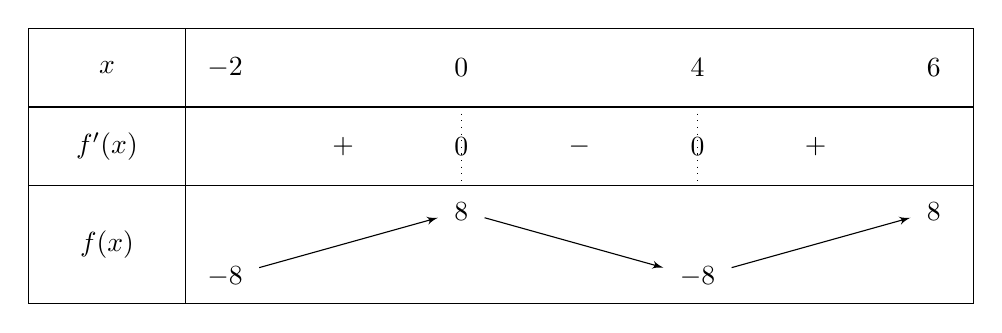
\begin{tikzpicture}
            \tkzTabInit{$x$ / 1 , $f'(x)$ / 1, $f(x)$ / 1.5}{$-2$, $0$, $4$, $6$}
            \tkzTabLine{, +, z, -, z, +, }
            \tkzTabVar{-/ $-8$, +/ $8$, -/ $-8$, +/ $8$}
            \end{tikzpicture}
        } \\
        \textit{D'après le graphique et $f'(x) = 1,5x(x - 4)$.}
    \end{enumerate}

    \item
    \begin{enumerate}
        \item \reponse{$f'(x) = 1,5x(x - 4)$.} \\
        \textit{$f'(x) = 1,5x^2 - 6x = 1,5x(x - 4)$.}

        \item \reponse{$f'(x) > 0$ sur $[-2; 0]$ et $[4; 6]$, $f'(x) < 0$ sur $[0; 4]$.} \\
        \textit{$f'(x) = 0$ pour $x = 0$ et $x = 4$.}
    \end{enumerate}

    \item \reponse{La courbe $\mathcal{C}$ est en dessous de $T$ sur $[0; 2]$.} \\
    \textit{$f(x) \leq -6x + 12$ sur $[0; 2]$.}
\end{enumerate}

\subsection*{Exercice 3 : Probabilités}

\begin{enumerate}
    \item
    \begin{enumerate}
        \item \reponse{Faux.} \\
        \textit{$P(\text{non dopé ou test positif}) = \frac{198}{200} = 0,99$.}

        \item \reponse{Vrai.} \\
        \textit{$P(\text{non dopé} \mid \text{test positif}) = \frac{15}{20} = 0,75$.}

        \item \reponse{Vrai.} \\
        \textit{$P(\text{erreur}) = \frac{17}{200} = 0,085$.}
    \end{enumerate}

    \item \reponse{Faux.} \\
    \textit{$P(\text{un succès}) = 2 \times 0,9 \times 0,1 = 0,18$.}
\end{enumerate}

\end{document}